
\chapter{Appendix}

\section{Dendritic leakage conductance}\label{sec-gl-dend}

In order to match the dendritic potential of rate neurons  in the spiking neuron model, a suitable leakage conductance
for dendritic compartments was required. As described in Equation \ref{eq-spiking-basal-compartment}, a dendritic
compartment evolves according to:
\begin{align}
  C_m^{dend} \dot{v}_j^{dend} & = -g_l^{dend} \  v_j^{dend} + \sum_i W_{ji} \    \langle \textit{n}_i \rangle
\end{align}

Under the assumption that the activation of all presynaptic neurons $i$ remains static over time, we can replace the
spontaneous activation $s_i(t)$ with the expected number of spikes per simulation step $\langle \textit{n}_i \rangle =
r_i \ \Delta t$ (cf. Equation \ref{eq-n-spikes}). Note that these values do not employ matrix notation, but refer to
individual neurons. Next, in order to find the convergence point of the ODE, we set the left side of the equation to $0$
and to solve it:

\begin{align}
  0                        & = -g_l^{dend} \  v_j^{dend} + \sum_i W_{ji} \    r_i \ \Delta t \\
  g_l^{dend} \  v_j^{dend} & = W_{ji} \    r_i \ \Delta t
\end{align}

The instantaneous dendritic potential of rate neurons is given by $v_j^{dend} = \sum_i W_{ji} \ r_i$. Since we are
searching for a parametrization which fulfills this equality in the steady state, the terms drop out from the above
equation. Thus, the correct parametrization for the dendritic leakage conductance remains:
\begin{align}
  g_l^{dend} & = \Delta t
\end{align}

It was shown experimentally that for high values of $\psi$, this parametrization leads to an exact match of dendritic
potentials between the neuron models. It will therefore be assumed as the default throughout all experiments where
spiking neurons are used. \newline

In order to keep the two NEST models as similar as possible, rate neurons evolve according to the same dynamics. Like in
the original implementation, dendrites of rate neurons ought to be fully defined by their inputs at time $t$. This
behavior is achieved by setting the leakage conductance to $1$ for all dendritic compartments. During network
initialization, dendritic leakage conductances are set to either one of these values depending on the type of neuron
model employed.


\section{Plasticity in feedback connections}\label{sec-feedback-plast}

Within the dendritic error model, Pyramidal-to-pyramidal feedback weights evolve according to:

\begin{align}
  \dot{w}_{l}^{down} & = \eta_l^{down} \ ( \phi(u_l^{P}) - \phi(w_l^{down} r_{l+1}^P) )\ \phi(u_{l+1}^{P})^T
\end{align}

The error term in this case differs slightly from the others, but could arguably still be implemented by biological
neurons. An intuitive way to interpret the error term is as the difference between somatic activity and the activity of
a distant apical compartment that is innervated only by superficial pyramidal neurons. The separation of pyramidal
neuron apical dendrites into a proximal and a distal tree is well documented \citep{Ishizuka1995}. Likewise, the fact
that these different apical compartments are innervated by separate presynaptic populations is established
\citep{Larkum2018}. A difference between plasticity mechanisms for synapses arriving at these two integration zones is
likewise plausible, as vastly different membrane dynamics and ion concentrations have been measured between them
\citep{Ishizuka1995,Larkum2022}. A more sophisticated model of the apical tree and its plasticity could therefore be a
desirable extension to the model.

While the plasticity was successfully implemented in all variants of the model, it did not prove useful for training the
networks during initial tests. Making these feedback connections non-plastic led to the best learning performance, and
is therefore assumed as the default for all training simulations. This matches the previous implementations of this
network, which typically set learning rates of these connections to $0$ except for a few experiments employing
steady-state approximations. Note that under these conditions the network effectively implements a type of Feedback
alignment \citep{Lillicrap2014}. Further work is required to identify why plasticity in these synapses seemed to break
learning in the present model.

\newpage
\section{Electronic supplementary material}

Attached to this thesis is a thumb drive containing the electronic supplementary material, which will briefly be
described here. The base directory contains a variant of the NEST simulator, which is published under the
\href{https://www.gnu.org/licenses/old-licenses/gpl-2.0.html}{GPLv2+} license. The NEST version included here was last
pulled from the public repository on December 20, 2022 and therefore lies somewhere between NEST 3.3 and 3.4. Under the
\texttt{models} directory, the neuron (\texttt{pp\_\allowbreak cond\_\allowbreak exp\_\allowbreak mc\_\allowbreak pyr},
\texttt{rate\_\allowbreak neuron\_\allowbreak pyr}) and synapse models (\texttt{pyr\_\allowbreak synapse},
\texttt{pyr\_\allowbreak synapse\_\allowbreak rate}) are located with corresponding \texttt{.cpp} and \texttt{.h} files.
Furthermore, the \texttt{pyr\_\allowbreak archiving\_\allowbreak node} responsible for storage and readout of dendritic
error, is located in the \texttt{nestkernel} directory. Other changes to the simulator largely serve to embed these
files and make them accessible from the PyNEST API.

The easiest way to compile the NEST simulator (which is required to run the model) is through conda. The
\texttt{requirements.txt} file in the base directory specifies the required packages. After creating a new environment
with\newline

\texttt{\$ conda create -n <environment-name> --file requirements.txt}\newline

a \href{https://nest-simulator.readthedocs.io/en/v3.4/installation/condaenv_install.html#condaenv}{guide from the NEST
documentation} should simplify setup of the simulator.

The project directory \texttt{dendritic\_\allowbreak error\_\allowbreak network} (roughly) follows the ``Good research
handbook`` \citep{Mineault2021}:

\begin{itemize}
  \item \textbf{data} contains all figures included in this thesis, as well as some additional ones.
  \item \textbf{results} contains all relevant simulation results. Parameter studies have their own subfolders, titled
  with the prefix \texttt{par\_study\_}. Each simulation stores its full parameter set (\texttt{params.json}), initial
  weights (\texttt{init\_weights.json}), final weights (\texttt{weights.json}) and training progress
  (\texttt{progress.json}). Intermediate weights are stored every few epochs during training in the \texttt{data}
  subdirectory. If plots were created to validate training progress, they are found in the \texttt{plots} folder.
  \item \textbf{experimental\_configs} contains JSON files to parameterize experiments. In these files, only the subset 
  of parameters needs to be specified which deviates from the default (cf. Supplementary table \ref{tab-params}).
  \item \textbf{scripts} contains scripts to be executed. The vast majority of them were written to validate individual
  assumptions made in this thesis. Of interest to perform experiments are \texttt{train\_network.py} and
  \texttt{parameter\_study.py}, which both support the \texttt{--help} parameter and will therefore not be detailed
  here.
  \item \textbf{src} contains a python module of reusable code (which should auto-install alongside the
  conda-environment). This includes networks, datasets, default parameters and some utilities.
  \item \textbf{tests} contains a test-suite which was used to validate the NEST implementation and fine-tune
  parameters. As it was only strictly necessary during the initial stages, it has not been updated throughout. Therefore
  most tests currently fail.
\end{itemize}


\newpage
\section{Supplementary Figures}


\renewcommand{\thefigure}{S\arabic{figure}}
\begin{figure}[h!]
  \centering
  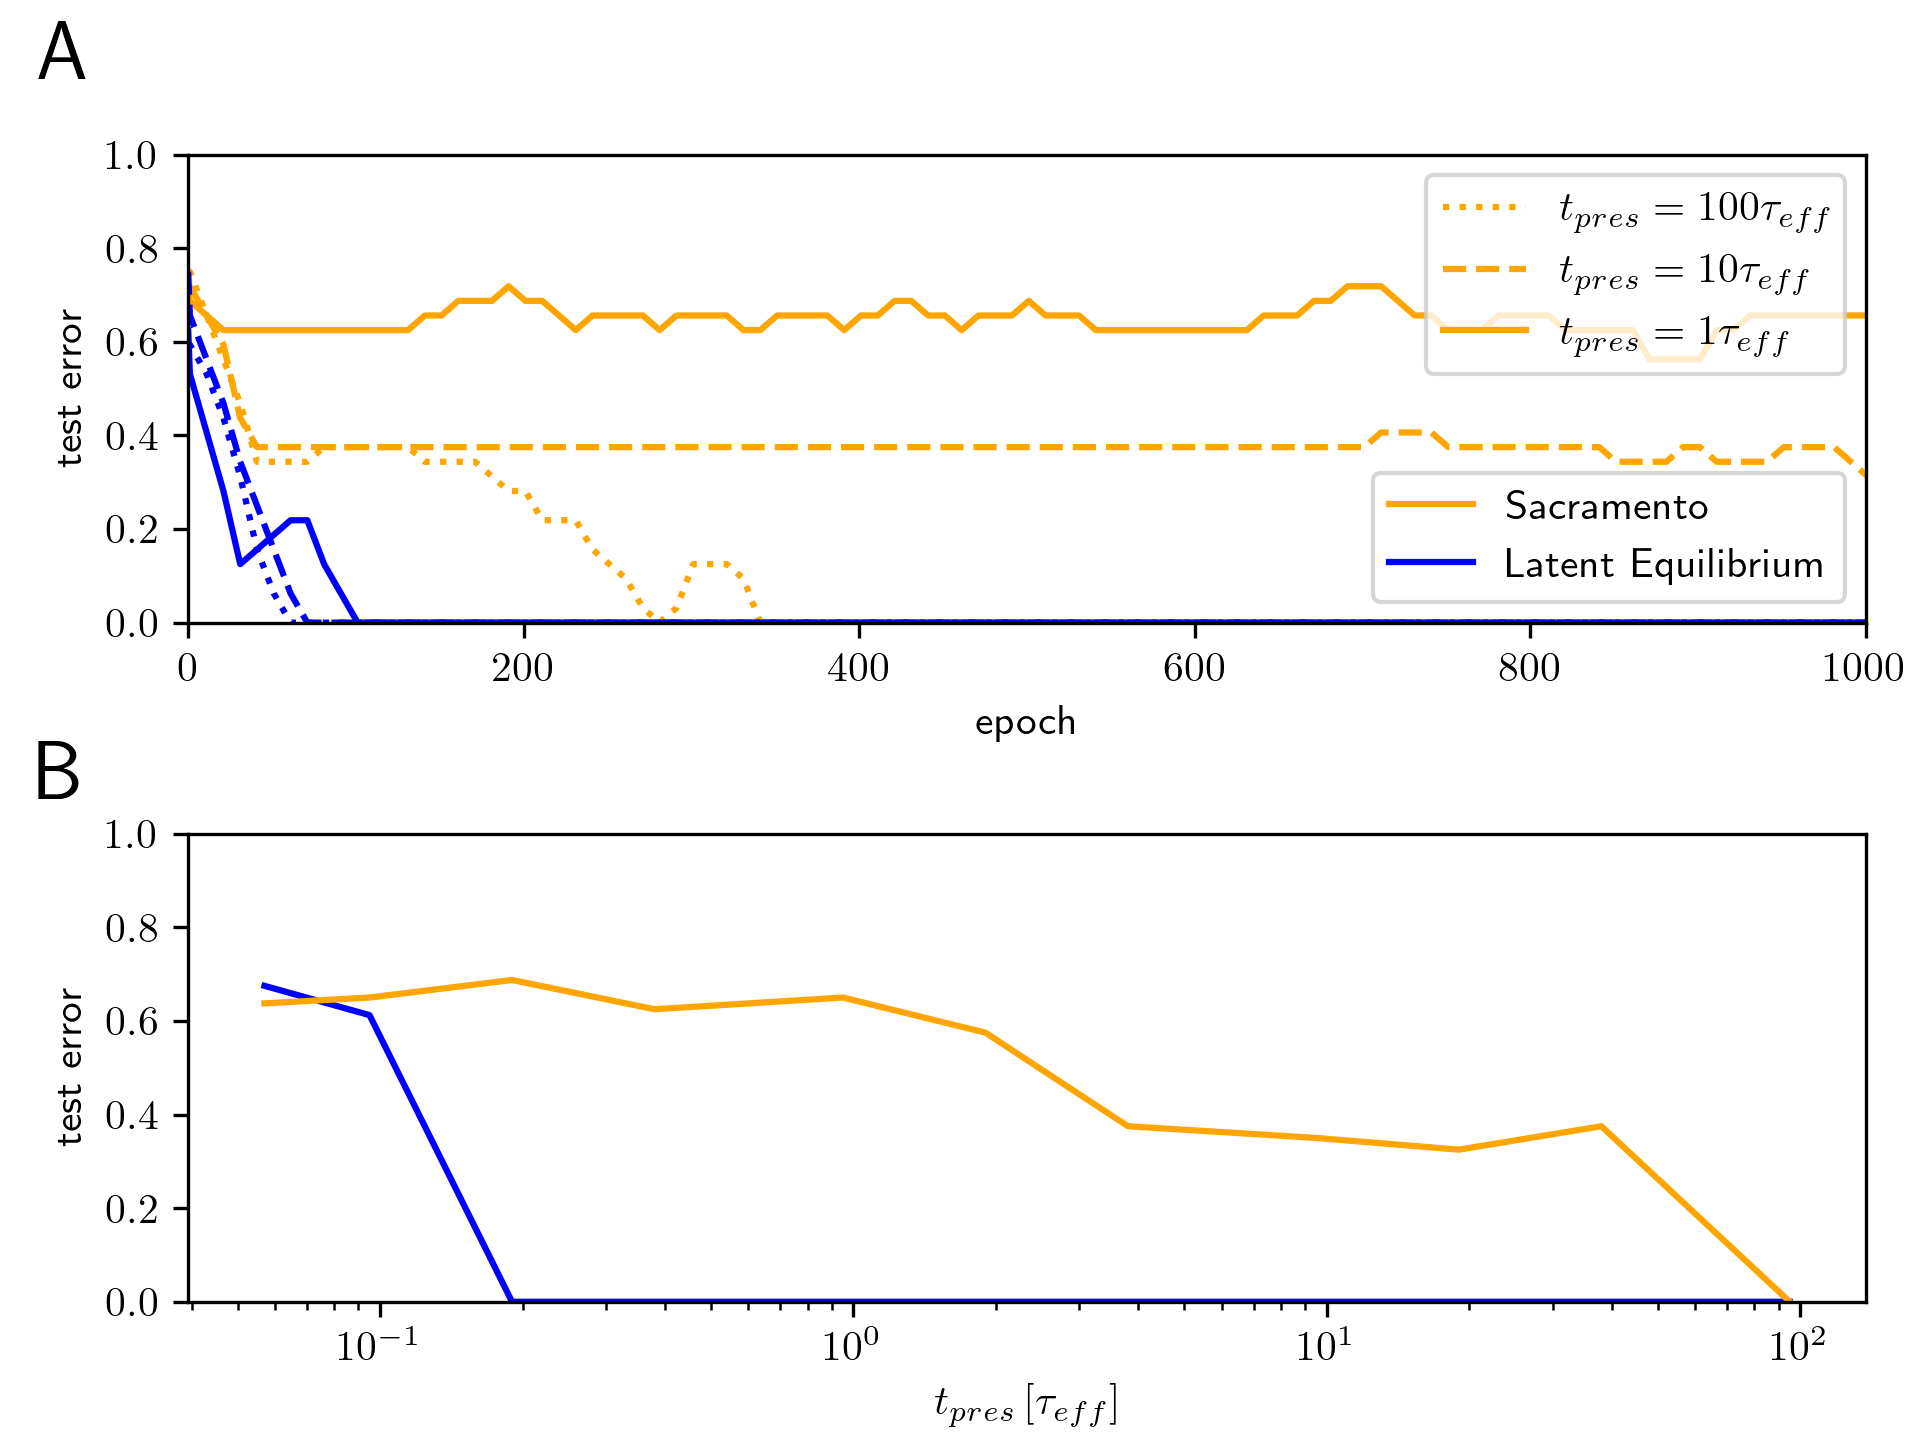
\includegraphics[width=0.9\textwidth]{fig_3_numpy}
  \caption[Replication of Fig. \ref{fig-bars-le-snest} using the NumPy network]{Replication of Fig.
    \ref{fig-bars-le-snest} using the NumPy network. This varaint is a slightly modified version of the python code from
    \citep{Haider2021}. Resulting performance matches the original results closely, showing that this version can serve
    as a baseline for comparing performance of the NEST implementation to the original results. Note, how in this
    implementation, presentation time has hardly any effect on the LE network because all updates are instantaneous. At
    the lower end presentation time is only limited by simulation timestep $\Delta t$.}
  \label{fig-bars-le-numpy}
\end{figure}


\begin{figure}[h!]
  \centering
  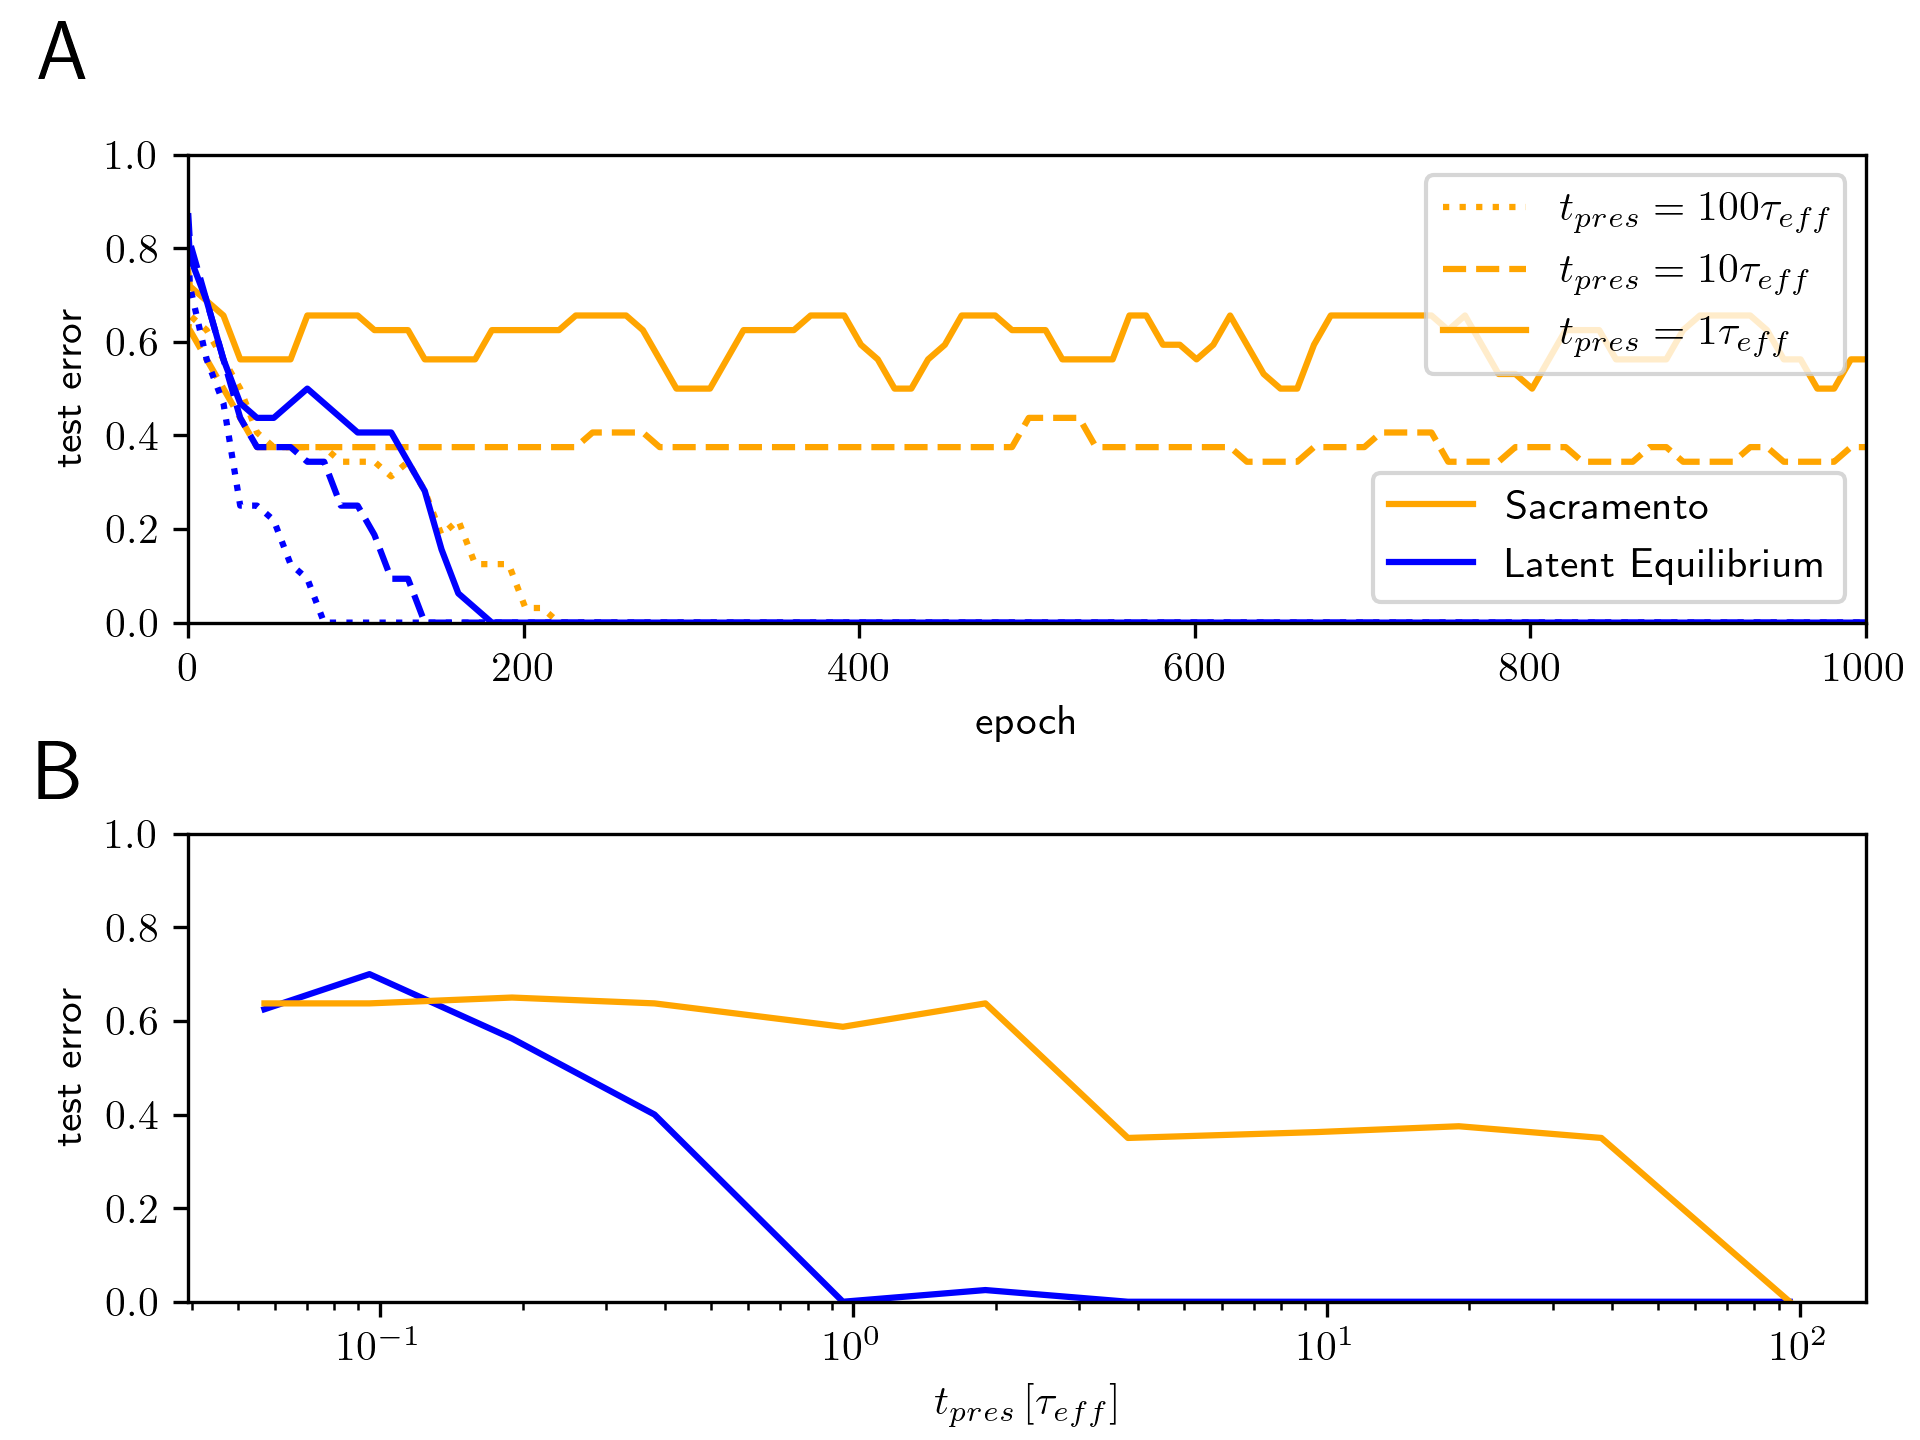
\includegraphics[width=0.9\textwidth]{fig_3_rnest}
  \caption[Replication of Fig. \ref{fig-bars-le-snest} using networks of rate neurons in the NEST simulator]{Replication
    of Fig. \ref{fig-bars-le-snest} using networks of rate neurons in the NEST simulator. A notable difference to the
    python implementation in Fig. \ref{fig-bars-le-numpy} is, that this version does not handle very low presentation
    times as well. This can likely be traced back to the synaptic delay enforced by NEST, which imposes an upper bound
    on network relaxation time. Besides that, performance of the two variants is very similar.}
  \label{fig-bars-le-rnest}
\end{figure}



\clearpage

\section{Supplementary Tables}



\renewcommand{\thetable}{S\arabic{table}}


\arrayrulecolor{white} % <--- {\renewcommand{\arraystretch}{1.45} 
\begin{table}[h]
  \resizebox{\textwidth}{!}{
    \begin{tabular}{|ll|ll|ll|} \hline \rowcolor[HTML]{B3B3B3} \multicolumn{2}{|l|}{\cellcolor[HTML]{B3B3B3}}
               & \multicolumn{2}{l|}{\cellcolor[HTML]{B3B3B3}Temporal-error model} &
               \multicolumn{2}{l|}{\cellcolor[HTML]{B3B3B3}Explicit-error model} \\
               \cline{3-6}
               \rowcolor[HTML]{B3B3B3}
               \multicolumn{2}{|l|}{\multirow{-2}{*}{\cellcolor[HTML]{B3B3B3}}}
               & \multicolumn{1}{l|}{\cellcolor[HTML]{B3B3B3}Contrastive learning} & Continuous update
               & \multicolumn{1}{l|}{\cellcolor[HTML]{B3B3B3}Predictive coding} & Dendritic error
               \\
               \hline
               \rowcolor[HTML]{D9D9D9} \multicolumn{2}{|l|}{\cellcolor[HTML]{D9D9D9}Control signal}
               &
               \multicolumn{1}{l|}{\cellcolor[HTML]{D9D9D9}{\color[HTML]{FE0000}
               Required}}
               & {\color[HTML]{FE0000} Required}
               &
               \multicolumn{1}{l|}{\cellcolor[HTML]{D9D9D9}{\color[HTML]{32CB00}
               Not required}}
               & {\color[HTML]{32CB00} Not required}
               \\ \hline
               \rowcolor[HTML]{D9D9D9}
               \multicolumn{2}{|l|}{\cellcolor[HTML]{D9D9D9}Connectivity}
               &
               \multicolumn{1}{l|}{\cellcolor[HTML]{D9D9D9}{\color[HTML]{32CB00}
               Unconstrained}}
                                                                                                                        &
                                                                                                                        {\color[HTML]{32CB00}
                                                                                                                        Unconstrained}
                                                                                                                        &
               \multicolumn{1}{l|}{\cellcolor[HTML]{D9D9D9}{\color[HTML]{FE0000}
               Constrained}}
               & {\color[HTML]{FE0000} Constrained} \\
               \hline
               \rowcolor[HTML]{D9D9D9}
               \multicolumn{2}{|l|}{\cellcolor[HTML]{D9D9D9}Propagation time} &
               \multicolumn{1}{l|}{\cellcolor[HTML]{D9D9D9}{\color[HTML]{32CB00}
               L-1}}
               & {\color[HTML]{32CB00} L-1}
               &
               \multicolumn{1}{l|}{\cellcolor[HTML]{D9D9D9}{\color[HTML]{FE0000}
               2L-1}}
               & {\color[HTML]{32CB00} L-1}
               \\
               \hline \rowcolor[HTML]{D9D9D9} \multicolumn{2}{|l|}{\cellcolor[HTML]{D9D9D9}Pre-training}
               &
               \multicolumn{1}{l|}{\cellcolor[HTML]{D9D9D9}{\color[HTML]{32CB00}
               Not required}}
               & {\color[HTML]{32CB00} Not required} &
               \multicolumn{1}{l|}{\cellcolor[HTML]{D9D9D9}{\color[HTML]{32CB00}
               Not required}}
               & {\color[HTML]{FE0000} Required} \\
               \hline
               \rowcolor[HTML]{D9D9D9}
               \multicolumn{2}{|l|}{\cellcolor[HTML]{D9D9D9}Error encoded in} &
                                                                                                                        \multicolumn{1}{l|}{\cellcolor[HTML]{D9D9D9}\begin{tabular}[c]{@{}l@{}}Difference
                                                                                                                        in
                                                                                                                        activity
                                                                                                                        \\
                                                                                                                                                                              between
                                                                                                                                                                              separate
                                                                                                                                                                              \\
                                                                                                                                                                              phases\end{tabular}}
                                                                                                                                                                              &
               \begin{tabular}[c]{@{}l@{}}Rate of change of \\
                     activity\end{tabular}                                                          &
               \multicolumn{1}{l|}{\cellcolor[HTML]{D9D9D9}\begin{tabular}[c]{@{}l@{}}Activity of specialised \\
                                                                   neurons\end{tabular}}                          &
               \begin{tabular}[c]{@{}l@{}}Apical dendrites of \\ pyramidal neurons\end{tabular}
               \\
               \hline \rowcolor[HTML]{D9D9D9} \multicolumn{2}{|l|}{\cellcolor[HTML]{D9D9D9}Data accounted for}
               & \multicolumn{1}{l|}{\cellcolor[HTML]{D9D9D9}\begin{tabular}[c]{@{}l@{}}Neural responses \\ and
               behaviour in a                         \\
                                                                   variety of tasks\end{tabular}} &
               \begin{tabular}[c]{@{}l@{}}Typical spike-time- \\ dependent plasticity\end{tabular}
               & \multicolumn{1}{l|}{\cellcolor[HTML]{D9D9D9}\begin{tabular}[c]{@{}l@{}}Increased neural \\
                                                                   activity to                  \\
                                                                   unpredicted stimuli\end{tabular}}               &
               \begin{tabular}[c]{@{}l@{}}Properties of \\
                     pyramidal neurons\end{tabular}
                     \\
               \hline \rowcolor[HTML]{D9D9D9} \multicolumn{2}{|l|}{\cellcolor[HTML]{D9D9D9}MNIST performance}
               & \multicolumn{1}{l|}{\cellcolor[HTML]{D9D9D9}$\sim$2-3}
               & -                                                                                                &
               \multicolumn{1}{l|}{\cellcolor[HTML]{D9D9D9}$\sim$1.7}
               & $\sim$1.96
               \\
               \hline
    \end{tabular}
  }\caption[Comparison between biologically plausible approximations of Backprop]{Comparison between biologically
    plausible approximations of Backprop, adapted from \citep{whittington2019theories}. From left to right: Contrastive
    hebbian learning \citep{OReilly1996}, Contrastive learing with continuous update \citep{Bengio2017}, Predictive
    coding network \citep{Whittington2017}, Dendritic error network \citep{sacramento2018dendritic}. All algorithms were
    selected because they reflect some properties of biological brains, some of which are highlighted in the row "Data
    accounted for". All of the algorithms need to make concessions for this. In the first four rows, desirable
    properties are highlighted in green, while undesirable traits are highlighted in red.}\label{tab-wb-models}

\end{table}


\begin{table}
  \fontsize{12pt}{12pt}\selectfont
  \begin{center}
    \begin{tabular}{p{0.25\textwidth}p{0.6\textwidth}p{0.15\textwidth}}    \hline
      \textbf{Name}                & \textbf{Description}                                                        &
      \textbf{Default}
      \\
      \hline

      \\\textbf{Simulation} \\\hline
      \texttt{n\_epochs}           & Number of training iterations                                               &
      $1000$ \\
      \texttt{delta\_t}            & Euler integration step in [ms]                                              & $0.1$
      \\
      \texttt{t\_pres}             & Stimulus presentation time during training [ms]                             & $50$
      \\
      \texttt{out\_lag}            & Delay before recording output during testing [ms]                           & $35$
      \\
      \texttt{dims}                & Network dimensions, i.e. pyramidal neurons per layer                        & [9,
          30, 3] \\
      \texttt{threads}             & Number of threads for parallel processing                                   & $8$
      \\
      \texttt{test\_interval}      & Test the network every N epochs                                             & $10$
      \\
      \texttt{record\_interval}    & Interval for storing membrane potentials [ms]                               & $1$
      \\
      \texttt{init\_self\_pred}    & Flag to initialize weights to self-predicting state                         &
      \texttt{True}
      \\
      \texttt{noise}               & Flag to apply noise to all somatic membrane potentials                      &
      \texttt{False}
      \\
      \texttt{sigma}               & Standard deviation for membrane potential noise                             & 0.3
      \\
      \texttt{mode}                & Which dataset to train on. Choice between (bars, mnist, self-pred, teacher) & bars
      \\
      \texttt{store\_errors}       & Flag to compute and store apical and interneuron errors during training     &
      \texttt{False}
      \\
      \texttt{network\_type}       & Choice between (numpy, snest, rnest)                                        & snest
      \\
      \texttt{tau\_x}              & Network input filtering time constant [ms]                                  & 0.1
      \\
      \texttt{reset}               & Reset method between simulations (0=no reset, 1=soft reset, 2=hard reset)   & 2
      \\

      \\
      \textbf{Neurons}
      \\\hline
      \texttt{latent\_equilibrium} & Flag for whether to use prospective transfer functions                      &
      \texttt{True}
      \\
      \texttt{g\_l}                & Somatic leakage conductance [nS]                                            & 0.03
      \\
      \texttt{g\_a}                & Apical compartment coupling conductance [nS]                                & 0.06
      \\
      \texttt{g\_d}                & Basal compartment coupling conductance [nS]                                 & 0.1
      \\
      \texttt{g\_som}              & Output neuron nudging conductance [nS]                                      & 0.06
      \\
      \texttt{g\_l\_eff}           & Effective leakage conductance [nS]                                          &
      \texttt{g\_l+g\_d+g\_a}
      \\
      \\
      \texttt{g\_lk\_dnd}          & Dendritic leakage [nS]                                                      &
      \texttt{delta\_t}
      \\
      \texttt{t\_ref}              & Refractory period [ms]                                                      & 0.0
      \\
      \texttt{C\_m\_som}           & Somatic compartment membrane capacitance [pF]                               & 1.0
      \\
      \texttt{C\_m\_bas}           & Basal compartment membrane capacitance [pF]                                 & 1.0
      \\
      \texttt{C\_m\_api}           & Apical compartment membrane capacitance [pF]                                & 1.0
      \\
      \texttt{gamma}               & Linearly scales  activation function $\phi$                                 & 1.0
      \\
      \texttt{beta}                & Exponentially scales  activation function $\phi$                            & 1.0
      \\
      \texttt{theta}               & Shifts  activation function $\phi$                                          & 0.0
      \\

      \\
      \textbf{Synapses}
      \\\hline
      \texttt{wmin\_init}          & Min. initial synaptic weight                                                & -1.0
      \\
      \texttt{wmax\_init}          & Max. initial synaptic weight                                                & 1.0
      \\
      \texttt{Wmin}                & Min. allowed synaptic weight                                                & -4.0
      \\
      \texttt{Wmax}                & Max. allowed synaptic weight                                                & 4.0
      \\
      \texttt{tau\_delta}          & Weight change filter time constant (NEST only) [ms]                         & 1.0
      \\

      \texttt{p\_conn}             & Connection probability between populations                                  & 1.0
      \\
      \texttt{eta\_ip}             & Learning rate for $pyr\rightarrow intn$ synapses                            & 0.004
      \\
      \texttt{eta\_pi}             & Learning rate for $intn\rightarrow pyr$ synapses                            & 0.01
      \\
      \texttt{eta\_up}             & Learning rates for feedforwarsd $pyr\rightarrow pyr$ synapses               &
      [0.01, 0.003] \\
      \texttt{eta\_down}           & Learning rate for feedback $pyr\rightarrow pyr$ synapses                    & 0.0
      \\
    \end{tabular}\caption{Default parameters for the dendritic error model. }\label{tab-params}
  \end{center}
\end{table}
